Process variation constitutes one of the major concerns of multiprocessor system designs \cite{chandrakasan2001, srivastava2010}.
A crucial implication of process variation is that it renders the key parameters of a technological process, \eg, the effective channel length, gate oxide thickness, and threshold voltage, as random quantities.
Therefore, the same workload applied to two ``identical'' dies can lead to two different power and, thus, temperature profiles since the dissipation of power and heat essentially depends on the aforementioned stochastic quantities.
Consequently, process variation leads to performance degradation in the best case and to severe faults or burnt silicon in the worst scenario.
Under these circumstances, uncertainty quantification \cite{xiu2010, eldred2009} has evolved into an indispensable asset of the multiprocessor system designs that can provide high guaranties on the efficiency and robustness of their products to the end user.

As an example, consider a quad-core architecture subjected to the uncertainty of the parameters that affect the leakage current.\footnote{The experimental setup is described in \sref{experimental-results}.}
Assume first that these parameters have nominal values. We can then simulate the system under a certain workload and observe the corresponding temperature profile.
The result, labeled as ``Nominal'', is depicted in \fref{motivation-curve} where, for clarity, only two curves, corresponding to two processors, are presented (the two bottom blue lines). It can be seen that the temperature is always below $70^{\circ}$C. Now, let us assume a mild deviation of the parameters from the nominal values and run the simulation once again.
The result is the ``Mild'' curves in \fref{motivation-curve} (the two middle orange lines); the maximal temperature is already above $80^{\circ}$C.
Finally, we repeat the experiment considering a severe deviation of the parameters and observe the curves labeled as ``Severe'' in \fref{motivation-curve} (the two top green lines); the maximal temperature is almost $110^{\circ}$C.
Imagine that the designer, when tuning the solution constrained by a maximal temperature of $80^\circ$C, was guided exclusively by the nominal parameters. In this case, even with mild deviations, the circuits might be burnt.
The amount of burnt circuits depends on the probability distribution of these deviations.
Such an uncertainty has to be addressed in order to pursue efficiency and robustness.
Nevertheless, the majority of the literature related to power-temperature analysis ignores this important aspect, \eg, \cite{rao2009, rai2011, thiele2011, ukhov2012}.

\begin{figure}[bl]
  \vspace{-1.0em}
  \centering
  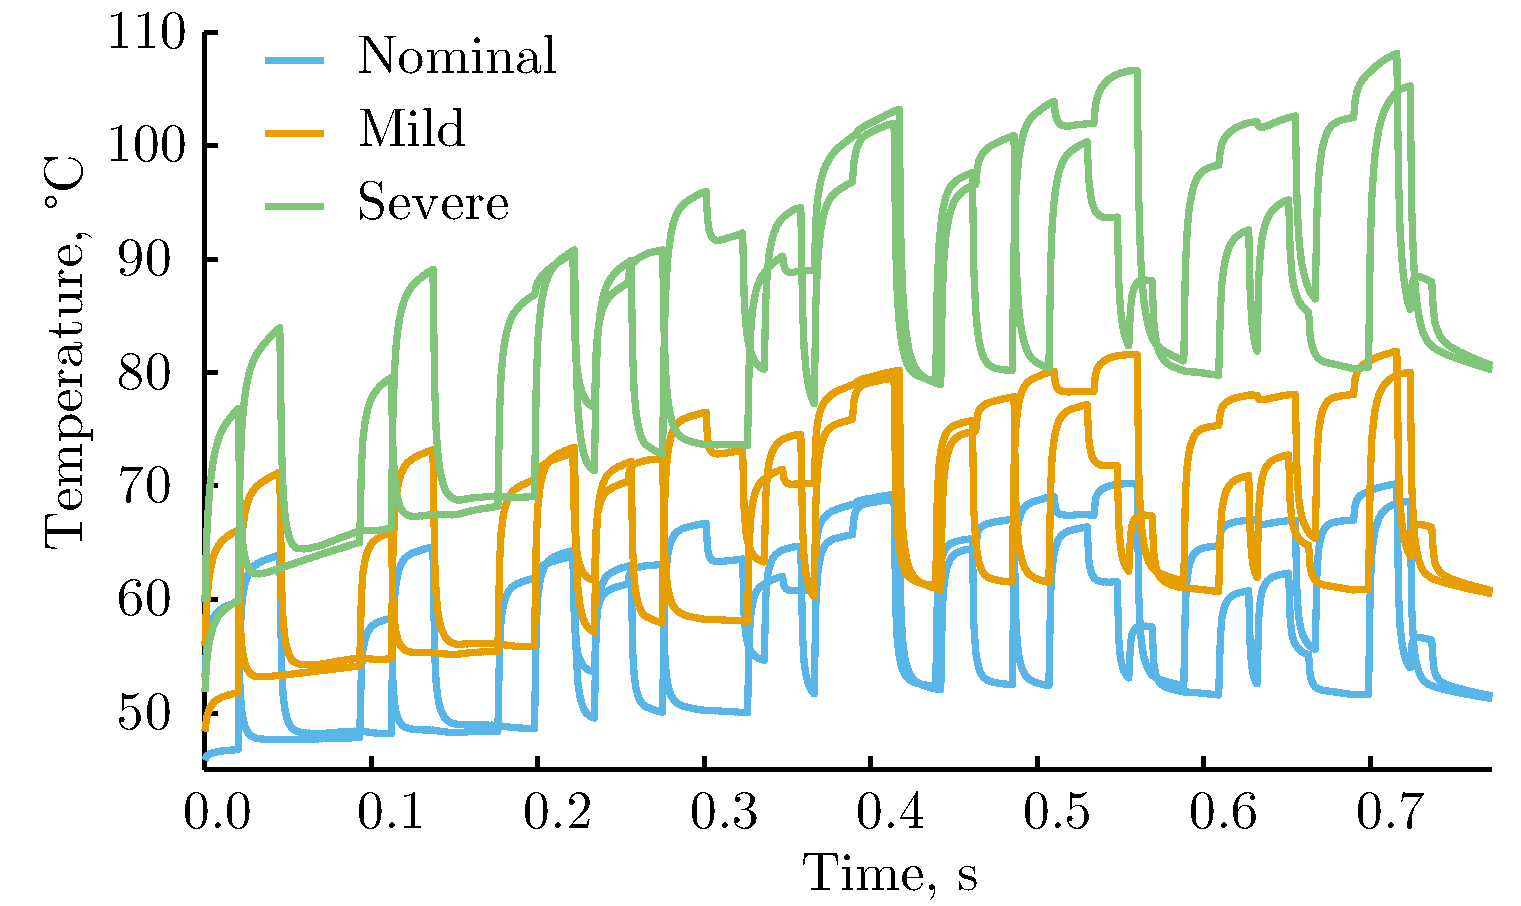
\includegraphics[width=1.0\linewidth]{include/assets/motivation-curve.pdf}
  \caption{Temperature fluctuation due to process variation.}
  \flabel{motivation-curve}
\end{figure}

\begin{figure}[br]
  \vspace{-1.5em}
  \centering
  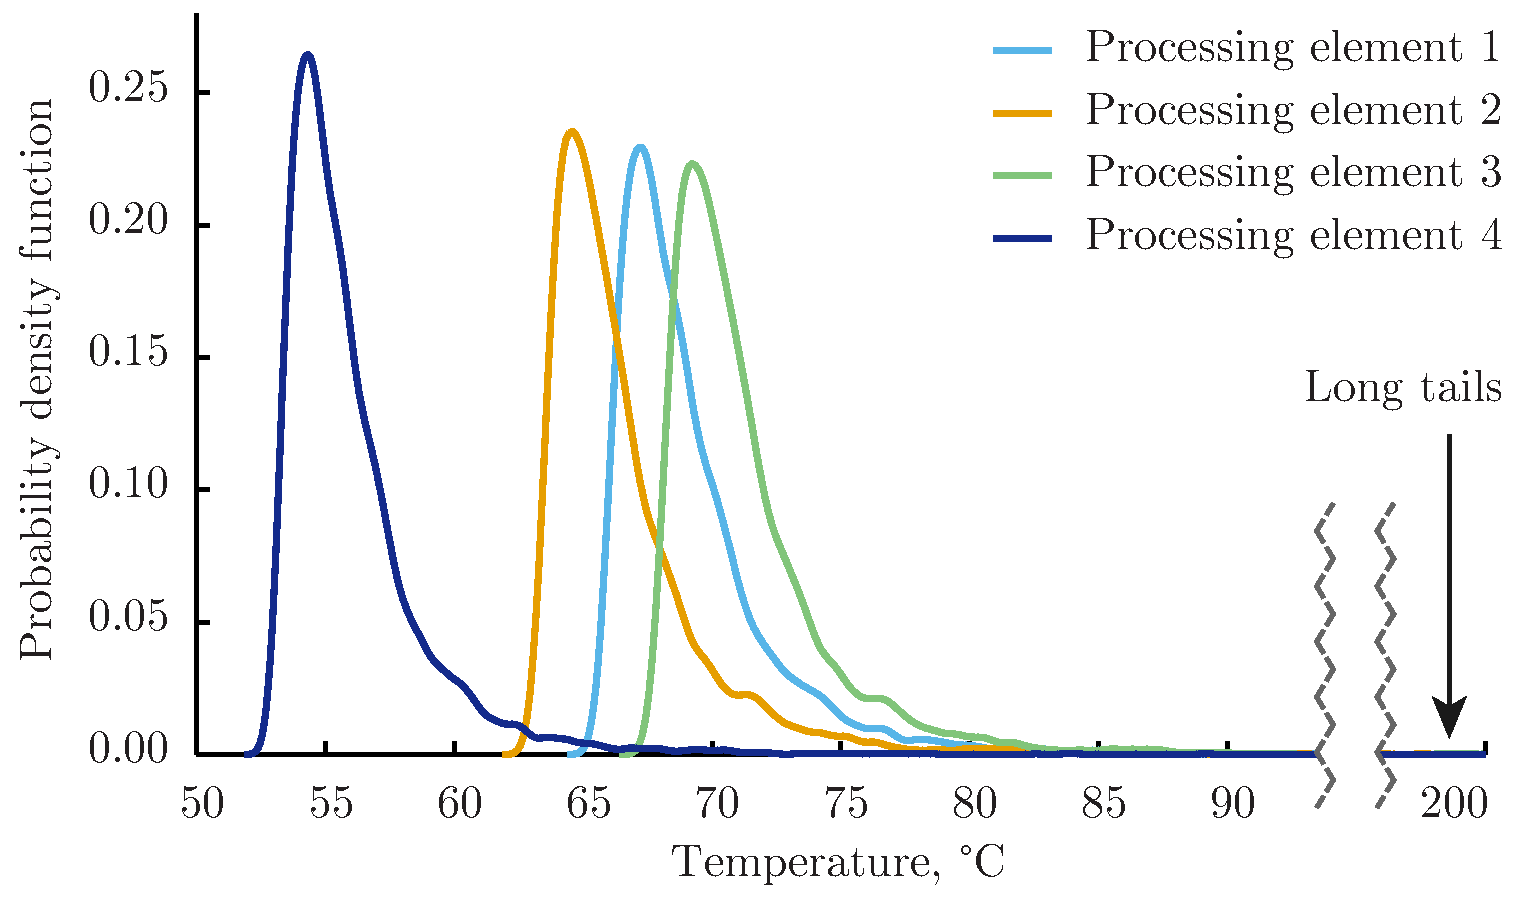
\includegraphics[width=1.0\linewidth]{include/assets/motivation-pdf.pdf}
  \caption{Probability density functions.}
  \flabel{motivation-pdf}
  \vspace{-1.0em}
\end{figure}

